
\chapter{Introduction and Background} 
\thispagestyle{myheadings} 
In this chapter, we first discuss some regular types of sensing systems 
used for guarding, tracking or surveilence, 
with a focus on the line-based and range-based sensors studied in this dissertation. 
% and we then introduce the two types of simplified sensing model studied in this thesis, 
Then, we conduct a literature study of the related work on sensor placement and 
coverage related problems. 
Lastly, some background knowledge of the theories and tools used in this paper will be given. 
\section{Some Examples of Sensing Systems} 
Sensor systems are ubiquitous. To list a few, systems of radar antennas 
or other sensor sources are frequently used as base stations for signal transmission, 
or intruder detection system (IDS) for monitoring hazards. 
The defense system can date back to ancient China where
watchtowers of the great wall are used as signal points when invaders appear. 
It can be seen as sensors from the broad sense
since ancient soldiers lit woods to create smoke and inform others when invaders appear. 
% Surveilence or tracking cameras surveillance and tracking system, 
\begin{figure}[ht]
    \centering 
    \begin{subfigure}[b]{0.281\textwidth} 
        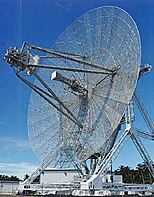
\includegraphics[width=\textwidth]{figures/Radar_antenna.jpg} 
        \caption{Radar antenna} 
        \label{fig:intro_radar} 
    \end{subfigure} 
    \begin{subfigure}[b]{0.48\textwidth} 
        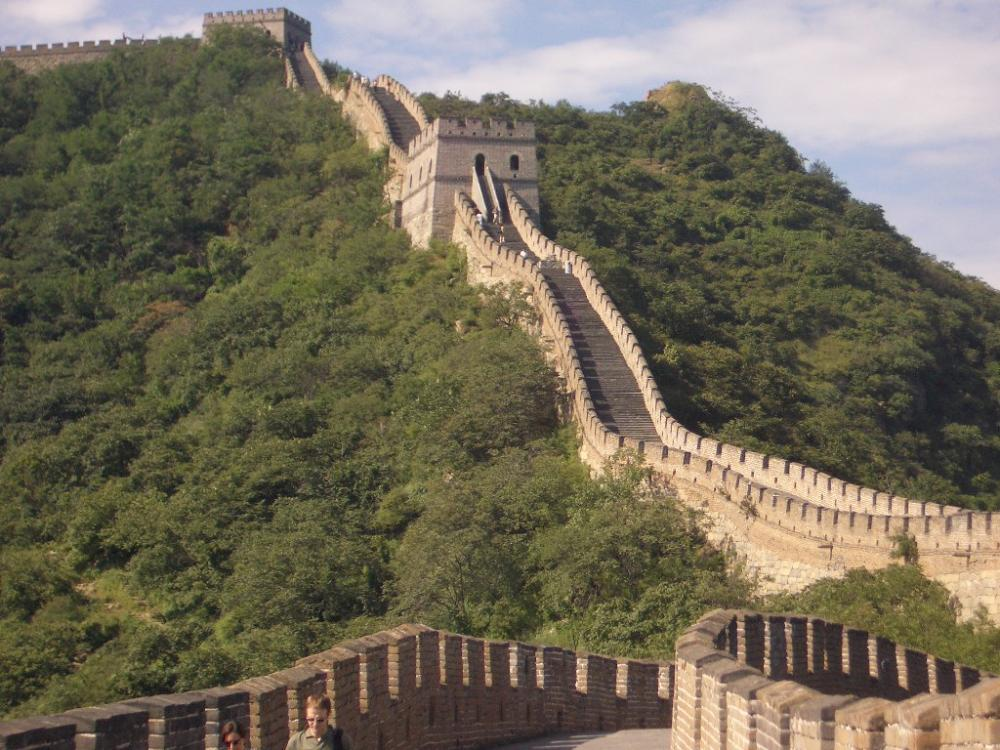
\includegraphics[width=\textwidth]{figures/great_wall.jpg} 
        \caption{The great wall of China} 
        \label{fig:intro_great_wall} 
    \end{subfigure} 
\end{figure}

On top of autonomous vehicles, sensor systems are indispensible for obstacle avoidance and interactions between vehicles, 
e.g., Tesla car (Fig.~\ref{fig:intro_tesla}) used 12 ultrasonic sensors 
near the front and rear bumper \footnote{\url{https://www.tesla.com/en_eu/support/transitioning-tesla-vision}}
and later changed into a vision system with only cameras. 
TuSimple, a truck company, employs a combination of cameras, radars and lidars 
for their perception system \footnote{\url{https://www.tusimple.com/blogs/tusimple-1000-meter-perception-system}}. 

\begin{figure}[ht] 
    \centering 

    \begin{subfigure}[b]{0.49\textwidth} 
        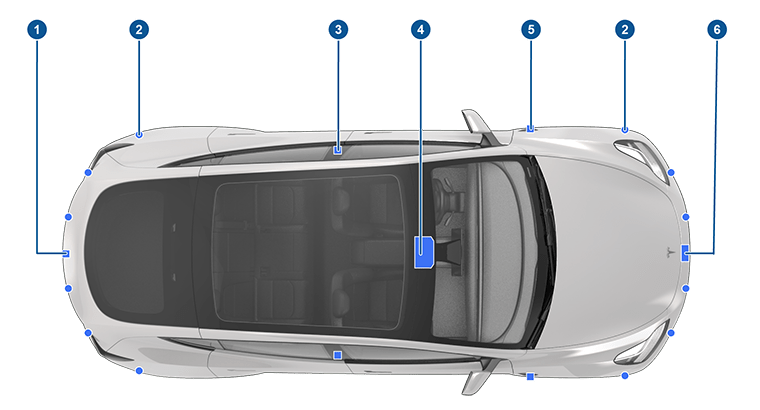
\includegraphics[width=\textwidth]{figures/tesla.png} 
        \caption{Tesla model Y's sensor system} 
        \label{fig:intro_tesla} 
    \end{subfigure} 
    \begin{subfigure}[b]{0.3\textwidth} 
        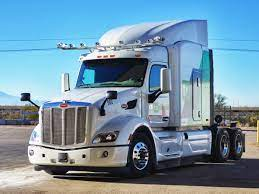
\includegraphics[width=\textwidth]{figures/truck_cam.jpeg} 
        \caption{TuSimple autonomous truck's sensor system} 
        \label{fig:intro_truckcam} 
    \end{subfigure} 
    
\end{figure} 

For surveilence or tracking systems, 
sensors like laser beams or cameras are deployed to detect thiefs. 
\begin{figure}[ht] 
    \centering 
    
    % \begin{subfigure}[b]{0.55\textwidth} 
    %     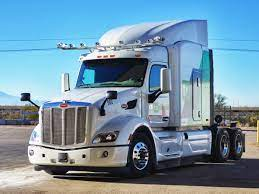
\includegraphics[width=\textwidth]{figures/truck_cam.jpeg} 
    %     \caption{Autonomous truck camera system} 
    %     \label{fig:intro_truckcam} 
    % \end{subfigure} 
    \begin{subfigure}[b]{0.41\textwidth} 
        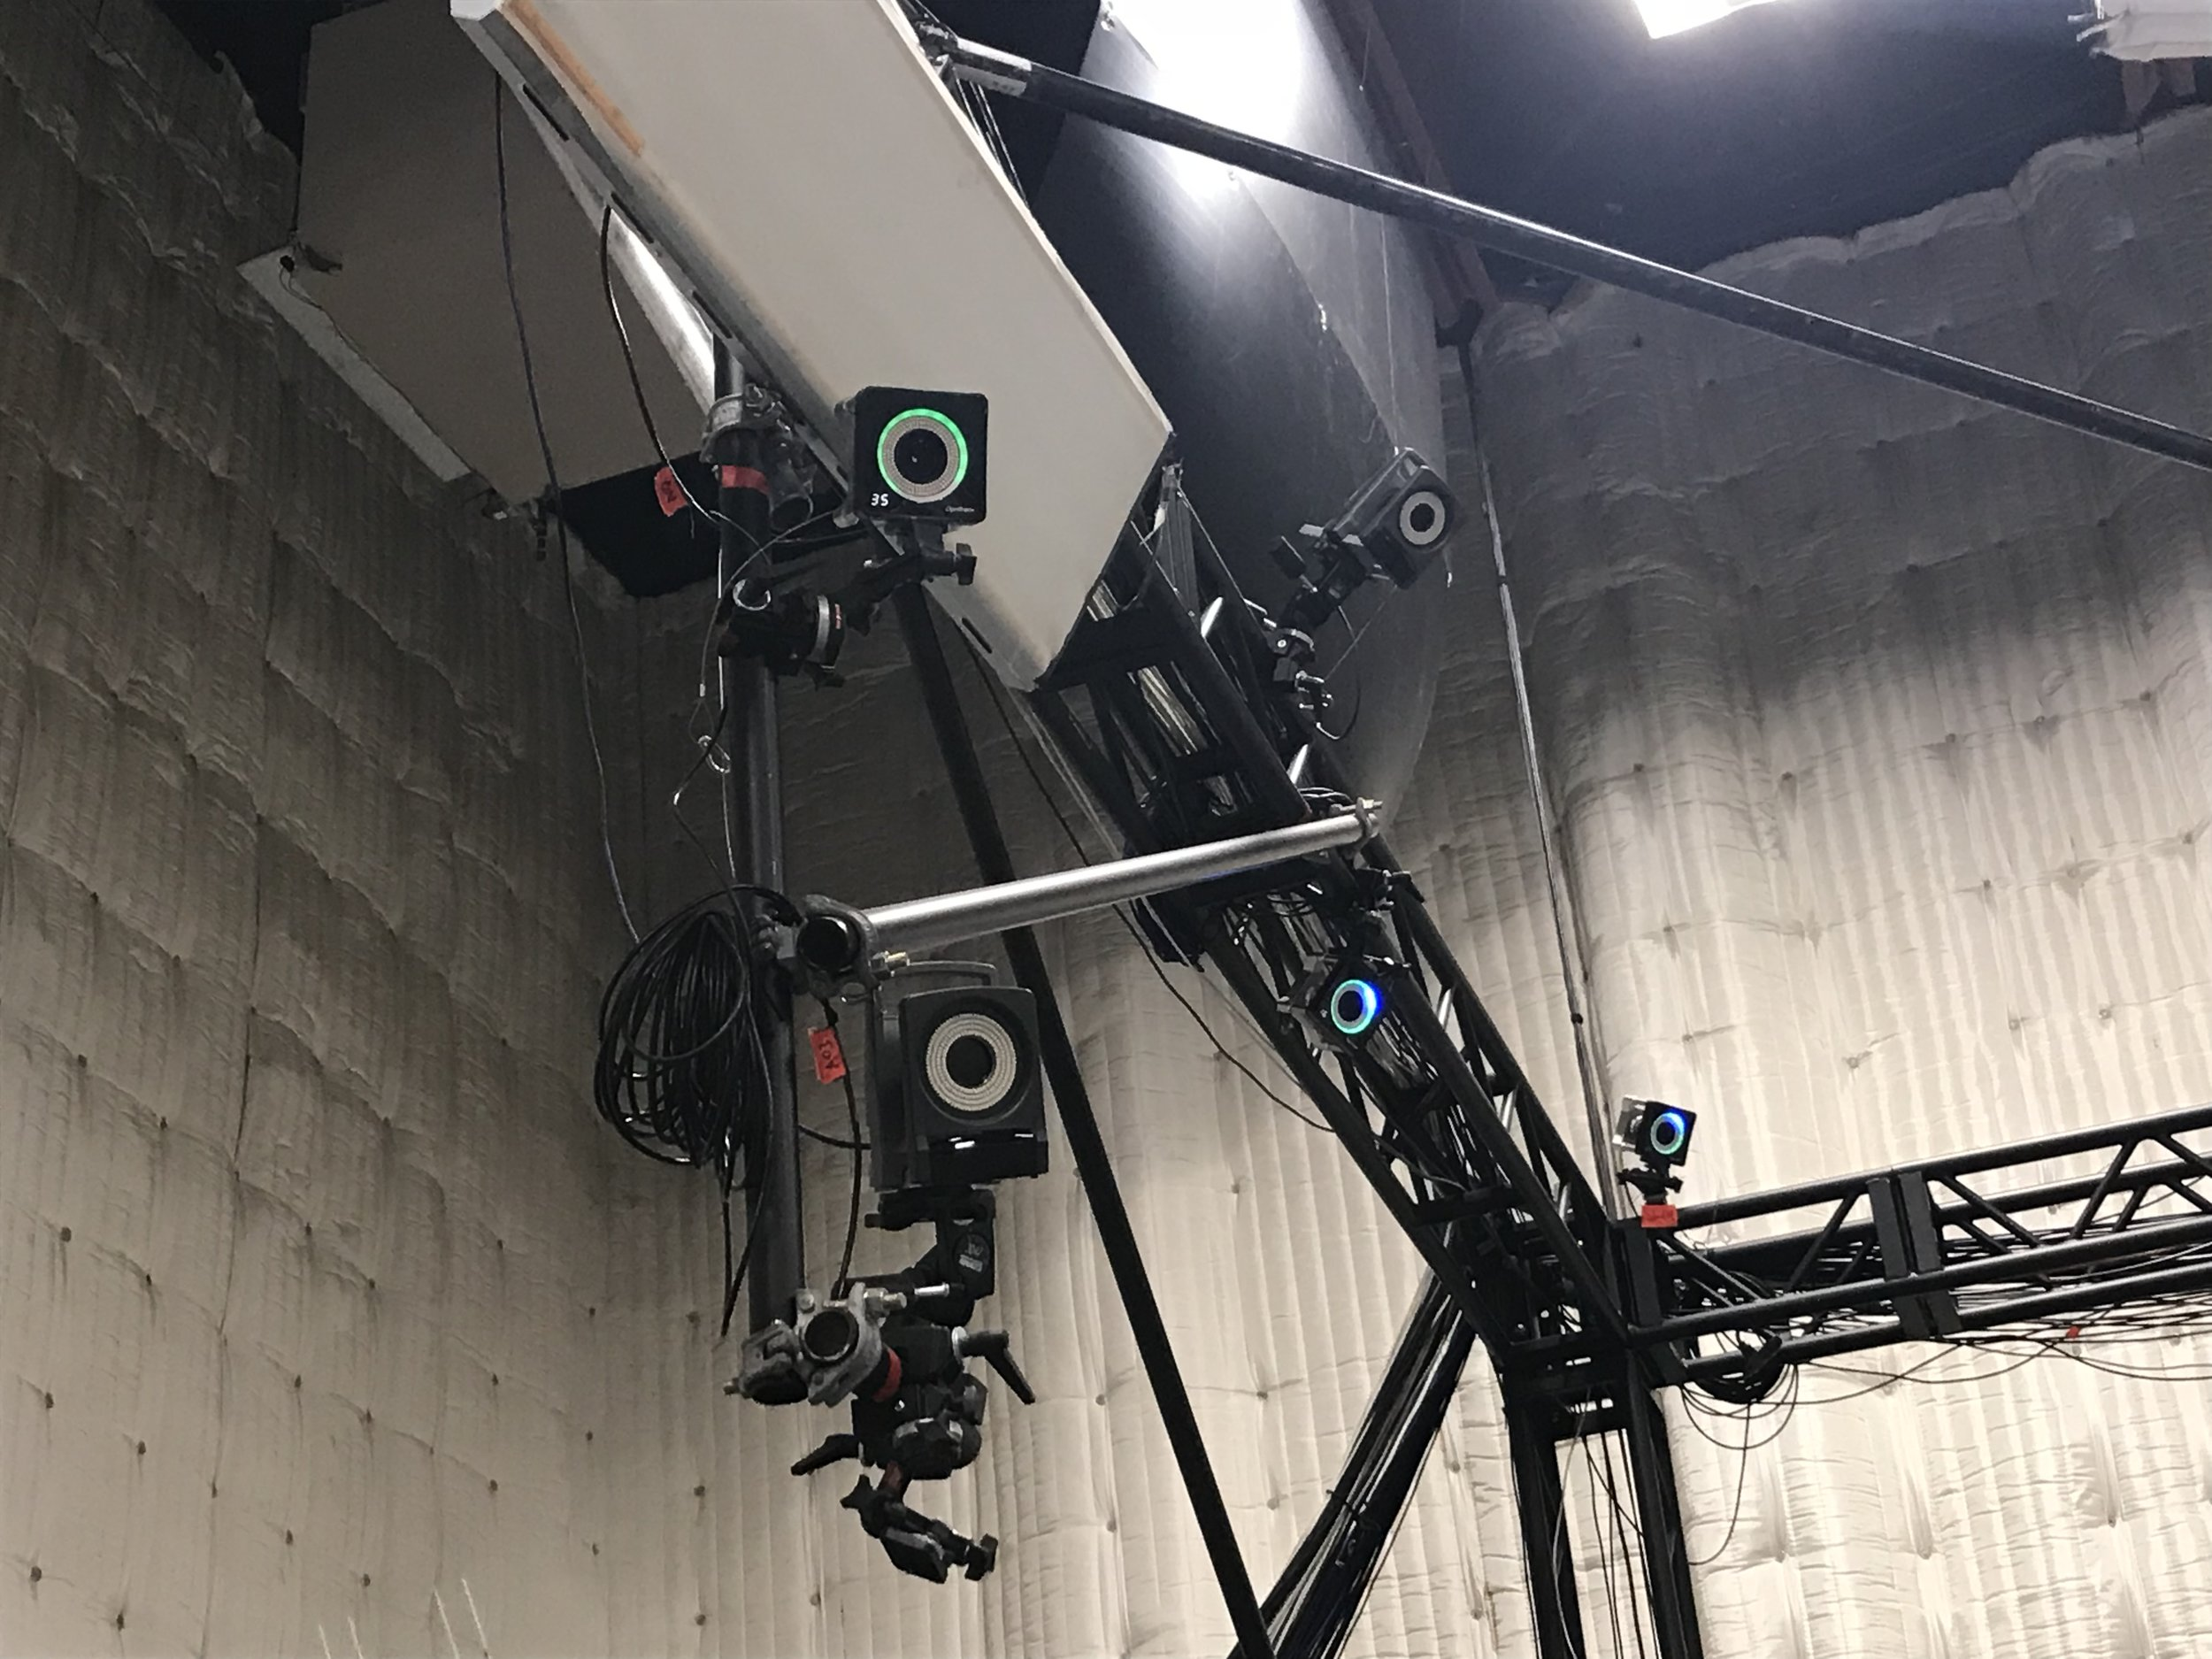
\includegraphics[width=\textwidth]{figures/optitrack.jpg} 
        \caption{Optical tracking system} 
        \label{fig:intro_optitrack} 
    \end{subfigure} 
    \begin{subfigure} [b]{0.46\textwidth} 
        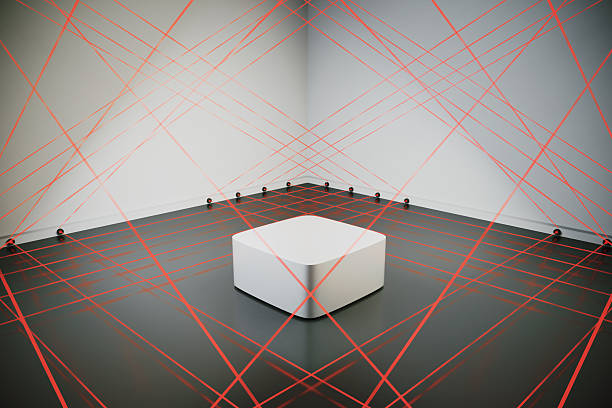
\includegraphics[width=\textwidth]{figures/laser.jpg} 
        \caption{Laser system} 
        \label{fig:intro_laser} 
    \end{subfigure} 
\end{figure} 

\section{Background}
\subsection{NP-hardness}
\subsection{Integer programming}
\section{Literature review} 
\subsection{Coverage-related problems in computational geometry} 

\subsection{Sensor network} 

\subsection{}
